%% main.tex — default manuscript entry point.
%% Build:  make            (draft)
%%         make submission (review-ready)
%% For a journal-specific build, use a thin wrapper that sets \ACTIVEJOURNAL
%% before %% main.tex — default manuscript entry point.
%% Build:  make            (draft)
%%         make submission (review-ready)
%% For a journal-specific build, use a thin wrapper that sets \ACTIVEJOURNAL
%% before %% main.tex — default manuscript entry point.
%% Build:  make            (draft)
%%         make submission (review-ready)
%% For a journal-specific build, use a thin wrapper that sets \ACTIVEJOURNAL
%% before %% main.tex — default manuscript entry point.
%% Build:  make            (draft)
%%         make submission (review-ready)
%% For a journal-specific build, use a thin wrapper that sets \ACTIVEJOURNAL
%% before \input{main.tex} — see templates/main-elife.tex.
\documentclass[draft]{cnnclab}

\addbibresource{refs.bib}

\title{A portable manuscript template for the publication lifecycle}
\author{R. Duarte\,\orcidlink{0000-0001-6099-667X}\textsuperscript{1,2}}
% CNC-UC researchers must use these two affiliations separately (see vault publication-rules).
\affiliation{1}{CNC-UC -- Center for Neuroscience and Cell Biology, University of Coimbra, 3004-504 Coimbra, Portugal}
\affiliation{2}{CIBB -- Centre for Innovative Biomedicine and Biotechnology, University of Coimbra, 3004-504 Coimbra, Portugal}
\corresponding{rcfduarte@gmail.com}
\keywords{computational neuroscience; reproducibility; manuscript preparation}
\runninghead{Publication-lifecycle template}

\begin{document}
\maketitle

\begin{abstract}
\sectioninput{abstract}
\end{abstract}

% Optional front-matter lay summary. Set the label per journal:
%   \significancelabel{Author Summary}      (PLOS)
%   \significancelabel{Significance}         (PNAS)
%   \significancelabel{New & Noteworthy}     (eNeuro)
% Default label is "Significance Statement" (J Neurosci / eNeuro style).
\begin{significance}
A short, lay-accessible statement of why this work matters (\textasciitilde75--200 words,
journal-dependent). Required by PLOS (Author Summary), J Neuroscience / eNeuro (Significance
Statement), and PNAS (Significance). Delete this block for journals that do not use it.
\end{significance}

\section{Introduction}\label{sec:intro}
\sectioninput{introduction}

\section{Results}\label{sec:results}
\sectioninput{results}

\section{Discussion}\label{sec:discussion}
\sectioninput{discussion}

\section{Methods}\label{sec:methods}
\sectioninput{methods}

\begin{acknowledgements}
% --- CiBB institutional references: MANDATORY in all CNC-UC/CiBB publications ---
This work was co-funded by the EU Recovery and Resilience Facility and Portuguese national
funds via FCT -- Fundação para a Ciência e a Tecnologia, under projects LA/P/0058/2020
[DOI: 10.54499/LA/P/0058/2020], UID/PRR/4539/2025 [DOI: 10.54499/UID/PRR/04539/2025] and
UID/04539/2025.
% --- Project-specific grant(s): replace with the reference(s) that fund your work ---
This work is funded by national funds via the FCT -- Foundation for Science and Technology,
I.P., under project 2023.13758.PEX (HetSyn).
\end{acknowledgements}
% Funding can instead be its own section: \begin{funding}...\end{funding}

% --- Back-matter statements required by most comp-neuro venues -----------------
\competinginterests{The authors declare no competing interests.}

\authorcontributions{% CRediT roles per author
  R.D.: Conceptualization, Methodology, Software, Formal analysis, Writing -- original draft.}

\dataavailability{All data supporting this study are available at
  \url{https://doi.org/10.5281/zenodo.XXXXXXX}.}

\codeavailability{Model and analysis code are available at
  \url{https://github.com/CNNC-Lab/...} and archived at
  \url{https://doi.org/10.5281/zenodo.XXXXXXX}.}

\printbibliography

% =============================================================================
% Supplementary material (after the bibliography). \beginsupplement flushes any
% deferred main figures first, then renumbers figures/tables/equations as S1, S2...
% =============================================================================
\beginsupplement

\suppsection{Supplementary Methods}
Additional methodological detail (e.g.\ full parameter tables, derivations, model
descriptions) that supports but is not essential to the main text.

\suppsection{Supplementary Figures}
\begin{figure}[htbp]
  \centering
  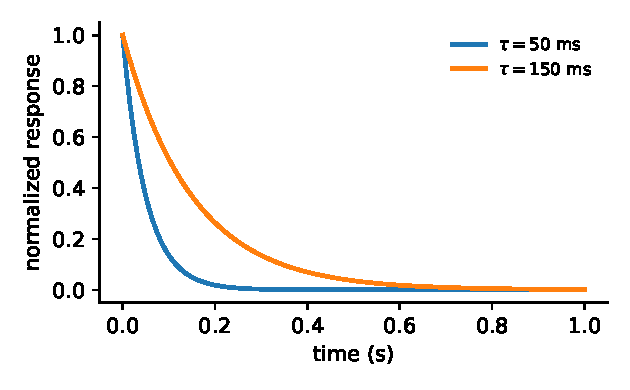
\includegraphics[width=0.5\linewidth]{figures/example-figure}
  \caption{\textbf{Supplementary example figure.} Numbered \cref{fig:supp-example}
    (i.e.\ Fig.~S1), independently of the main-text figures.}
  \label{fig:supp-example}
\end{figure}

\suppsection{Supplementary Tables}
\begin{table}[htbp]
  \centering
  \caption{\textbf{Supplementary example table.} Numbered \cref{tab:supp-example}
    (Table~S1). Parameter tables are the most common supplement in modelling papers.}
  \label{tab:supp-example}
  \begin{tabular}{lcc}
    \toprule
    Parameter & Symbol & Value \\
    \midrule
    Number of neurons   & $N$       & $10\,000$ \\
    Connection density  & $\epsilon$ & $0.1$ \\
    Synaptic delay      & $d$       & $1.5$ ms \\
    \bottomrule
  \end{tabular}
\end{table}

\end{document}
 — see templates/main-elife.tex.
\documentclass[draft]{cnnclab}

\addbibresource{refs.bib}

\title{A portable manuscript template for the publication lifecycle}
\author{R. Duarte\,\orcidlink{0000-0001-6099-667X}\textsuperscript{1,2}}
% CNC-UC researchers must use these two affiliations separately (see vault publication-rules).
\affiliation{1}{CNC-UC -- Center for Neuroscience and Cell Biology, University of Coimbra, 3004-504 Coimbra, Portugal}
\affiliation{2}{CIBB -- Centre for Innovative Biomedicine and Biotechnology, University of Coimbra, 3004-504 Coimbra, Portugal}
\corresponding{rcfduarte@gmail.com}
\keywords{computational neuroscience; reproducibility; manuscript preparation}
\runninghead{Publication-lifecycle template}

\begin{document}
\maketitle

\begin{abstract}
\sectioninput{abstract}
\end{abstract}

% Optional front-matter lay summary. Set the label per journal:
%   \significancelabel{Author Summary}      (PLOS)
%   \significancelabel{Significance}         (PNAS)
%   \significancelabel{New & Noteworthy}     (eNeuro)
% Default label is "Significance Statement" (J Neurosci / eNeuro style).
\begin{significance}
A short, lay-accessible statement of why this work matters (\textasciitilde75--200 words,
journal-dependent). Required by PLOS (Author Summary), J Neuroscience / eNeuro (Significance
Statement), and PNAS (Significance). Delete this block for journals that do not use it.
\end{significance}

\section{Introduction}\label{sec:intro}
\sectioninput{introduction}

\section{Results}\label{sec:results}
\sectioninput{results}

\section{Discussion}\label{sec:discussion}
\sectioninput{discussion}

\section{Methods}\label{sec:methods}
\sectioninput{methods}

\begin{acknowledgements}
% --- CiBB institutional references: MANDATORY in all CNC-UC/CiBB publications ---
This work was co-funded by the EU Recovery and Resilience Facility and Portuguese national
funds via FCT -- Fundação para a Ciência e a Tecnologia, under projects LA/P/0058/2020
[DOI: 10.54499/LA/P/0058/2020], UID/PRR/4539/2025 [DOI: 10.54499/UID/PRR/04539/2025] and
UID/04539/2025.
% --- Project-specific grant(s): replace with the reference(s) that fund your work ---
This work is funded by national funds via the FCT -- Foundation for Science and Technology,
I.P., under project 2023.13758.PEX (HetSyn).
\end{acknowledgements}
% Funding can instead be its own section: \begin{funding}...\end{funding}

% --- Back-matter statements required by most comp-neuro venues -----------------
\competinginterests{The authors declare no competing interests.}

\authorcontributions{% CRediT roles per author
  R.D.: Conceptualization, Methodology, Software, Formal analysis, Writing -- original draft.}

\dataavailability{All data supporting this study are available at
  \url{https://doi.org/10.5281/zenodo.XXXXXXX}.}

\codeavailability{Model and analysis code are available at
  \url{https://github.com/CNNC-Lab/...} and archived at
  \url{https://doi.org/10.5281/zenodo.XXXXXXX}.}

\printbibliography

% =============================================================================
% Supplementary material (after the bibliography). \beginsupplement flushes any
% deferred main figures first, then renumbers figures/tables/equations as S1, S2...
% =============================================================================
\beginsupplement

\suppsection{Supplementary Methods}
Additional methodological detail (e.g.\ full parameter tables, derivations, model
descriptions) that supports but is not essential to the main text.

\suppsection{Supplementary Figures}
\begin{figure}[htbp]
  \centering
  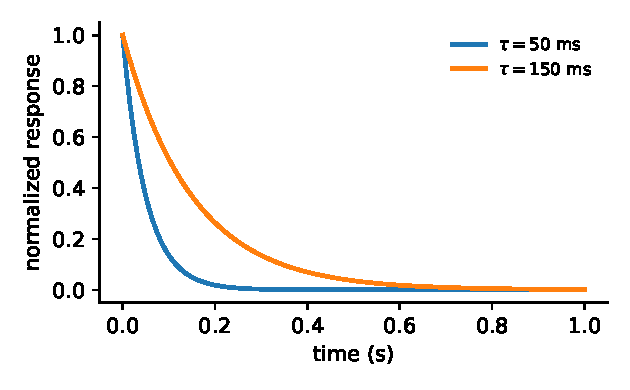
\includegraphics[width=0.5\linewidth]{figures/example-figure}
  \caption{\textbf{Supplementary example figure.} Numbered \cref{fig:supp-example}
    (i.e.\ Fig.~S1), independently of the main-text figures.}
  \label{fig:supp-example}
\end{figure}

\suppsection{Supplementary Tables}
\begin{table}[htbp]
  \centering
  \caption{\textbf{Supplementary example table.} Numbered \cref{tab:supp-example}
    (Table~S1). Parameter tables are the most common supplement in modelling papers.}
  \label{tab:supp-example}
  \begin{tabular}{lcc}
    \toprule
    Parameter & Symbol & Value \\
    \midrule
    Number of neurons   & $N$       & $10\,000$ \\
    Connection density  & $\epsilon$ & $0.1$ \\
    Synaptic delay      & $d$       & $1.5$ ms \\
    \bottomrule
  \end{tabular}
\end{table}

\end{document}
 — see templates/main-elife.tex.
\documentclass[draft]{cnnclab}

\addbibresource{refs.bib}

\title{A portable manuscript template for the publication lifecycle}
\author{R. Duarte\,\orcidlink{0000-0001-6099-667X}\textsuperscript{1,2}}
% CNC-UC researchers must use these two affiliations separately (see vault publication-rules).
\affiliation{1}{CNC-UC -- Center for Neuroscience and Cell Biology, University of Coimbra, 3004-504 Coimbra, Portugal}
\affiliation{2}{CIBB -- Centre for Innovative Biomedicine and Biotechnology, University of Coimbra, 3004-504 Coimbra, Portugal}
\corresponding{rcfduarte@gmail.com}
\keywords{computational neuroscience; reproducibility; manuscript preparation}
\runninghead{Publication-lifecycle template}

\begin{document}
\maketitle

\begin{abstract}
\sectioninput{abstract}
\end{abstract}

% Optional front-matter lay summary. Set the label per journal:
%   \significancelabel{Author Summary}      (PLOS)
%   \significancelabel{Significance}         (PNAS)
%   \significancelabel{New & Noteworthy}     (eNeuro)
% Default label is "Significance Statement" (J Neurosci / eNeuro style).
\begin{significance}
A short, lay-accessible statement of why this work matters (\textasciitilde75--200 words,
journal-dependent). Required by PLOS (Author Summary), J Neuroscience / eNeuro (Significance
Statement), and PNAS (Significance). Delete this block for journals that do not use it.
\end{significance}

\section{Introduction}\label{sec:intro}
\sectioninput{introduction}

\section{Results}\label{sec:results}
\sectioninput{results}

\section{Discussion}\label{sec:discussion}
\sectioninput{discussion}

\section{Methods}\label{sec:methods}
\sectioninput{methods}

\begin{acknowledgements}
% --- CiBB institutional references: MANDATORY in all CNC-UC/CiBB publications ---
This work was co-funded by the EU Recovery and Resilience Facility and Portuguese national
funds via FCT -- Fundação para a Ciência e a Tecnologia, under projects LA/P/0058/2020
[DOI: 10.54499/LA/P/0058/2020], UID/PRR/4539/2025 [DOI: 10.54499/UID/PRR/04539/2025] and
UID/04539/2025.
% --- Project-specific grant(s): replace with the reference(s) that fund your work ---
This work is funded by national funds via the FCT -- Foundation for Science and Technology,
I.P., under project 2023.13758.PEX (HetSyn).
\end{acknowledgements}
% Funding can instead be its own section: \begin{funding}...\end{funding}

% --- Back-matter statements required by most comp-neuro venues -----------------
\competinginterests{The authors declare no competing interests.}

\authorcontributions{% CRediT roles per author
  R.D.: Conceptualization, Methodology, Software, Formal analysis, Writing -- original draft.}

\dataavailability{All data supporting this study are available at
  \url{https://doi.org/10.5281/zenodo.XXXXXXX}.}

\codeavailability{Model and analysis code are available at
  \url{https://github.com/CNNC-Lab/...} and archived at
  \url{https://doi.org/10.5281/zenodo.XXXXXXX}.}

\printbibliography

% =============================================================================
% Supplementary material (after the bibliography). \beginsupplement flushes any
% deferred main figures first, then renumbers figures/tables/equations as S1, S2...
% =============================================================================
\beginsupplement

\suppsection{Supplementary Methods}
Additional methodological detail (e.g.\ full parameter tables, derivations, model
descriptions) that supports but is not essential to the main text.

\suppsection{Supplementary Figures}
\begin{figure}[htbp]
  \centering
  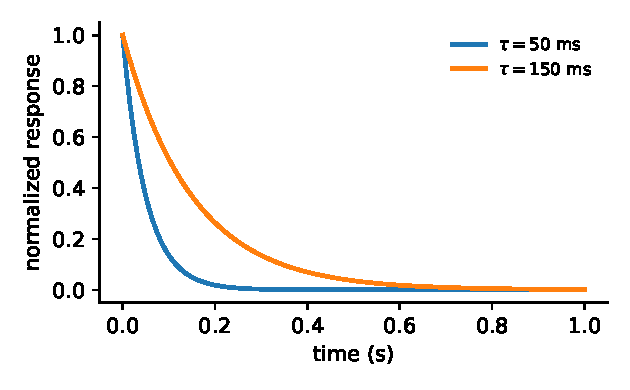
\includegraphics[width=0.5\linewidth]{figures/example-figure}
  \caption{\textbf{Supplementary example figure.} Numbered \cref{fig:supp-example}
    (i.e.\ Fig.~S1), independently of the main-text figures.}
  \label{fig:supp-example}
\end{figure}

\suppsection{Supplementary Tables}
\begin{table}[htbp]
  \centering
  \caption{\textbf{Supplementary example table.} Numbered \cref{tab:supp-example}
    (Table~S1). Parameter tables are the most common supplement in modelling papers.}
  \label{tab:supp-example}
  \begin{tabular}{lcc}
    \toprule
    Parameter & Symbol & Value \\
    \midrule
    Number of neurons   & $N$       & $10\,000$ \\
    Connection density  & $\epsilon$ & $0.1$ \\
    Synaptic delay      & $d$       & $1.5$ ms \\
    \bottomrule
  \end{tabular}
\end{table}

\end{document}
 — see templates/main-elife.tex.
\documentclass[draft]{cnnclab}

\addbibresource{refs.bib}

\title{A portable manuscript template for the publication lifecycle}
\author{R. Duarte\,\orcidlink{0000-0001-6099-667X}\textsuperscript{1,2}}
% CNC-UC researchers must use these two affiliations separately (see vault publication-rules).
\affiliation{1}{CNC-UC -- Center for Neuroscience and Cell Biology, University of Coimbra, 3004-504 Coimbra, Portugal}
\affiliation{2}{CIBB -- Centre for Innovative Biomedicine and Biotechnology, University of Coimbra, 3004-504 Coimbra, Portugal}
\corresponding{rcfduarte@gmail.com}
\keywords{computational neuroscience; reproducibility; manuscript preparation}
\runninghead{Publication-lifecycle template}

\begin{document}
\maketitle

\begin{abstract}
\sectioninput{abstract}
\end{abstract}

% Optional front-matter lay summary. Set the label per journal:
%   \significancelabel{Author Summary}      (PLOS)
%   \significancelabel{Significance}         (PNAS)
%   \significancelabel{New & Noteworthy}     (eNeuro)
% Default label is "Significance Statement" (J Neurosci / eNeuro style).
\begin{significance}
A short, lay-accessible statement of why this work matters (\textasciitilde75--200 words,
journal-dependent). Required by PLOS (Author Summary), J Neuroscience / eNeuro (Significance
Statement), and PNAS (Significance). Delete this block for journals that do not use it.
\end{significance}

\section{Introduction}\label{sec:intro}
\sectioninput{introduction}

\section{Results}\label{sec:results}
\sectioninput{results}

\section{Discussion}\label{sec:discussion}
\sectioninput{discussion}

\section{Methods}\label{sec:methods}
\sectioninput{methods}

\begin{acknowledgements}
% --- CiBB institutional references: MANDATORY in all CNC-UC/CiBB publications ---
This work was co-funded by the EU Recovery and Resilience Facility and Portuguese national
funds via FCT -- Fundação para a Ciência e a Tecnologia, under projects LA/P/0058/2020
[DOI: 10.54499/LA/P/0058/2020], UID/PRR/4539/2025 [DOI: 10.54499/UID/PRR/04539/2025] and
UID/04539/2025.
% --- Project-specific grant(s): replace with the reference(s) that fund your work ---
This work is funded by national funds via the FCT -- Foundation for Science and Technology,
I.P., under project 2023.13758.PEX (HetSyn).
\end{acknowledgements}
% Funding can instead be its own section: \begin{funding}...\end{funding}

% --- Back-matter statements required by most comp-neuro venues -----------------
\competinginterests{The authors declare no competing interests.}

\authorcontributions{% CRediT roles per author
  R.D.: Conceptualization, Methodology, Software, Formal analysis, Writing -- original draft.}

\dataavailability{All data supporting this study are available at
  \url{https://doi.org/10.5281/zenodo.XXXXXXX}.}

\codeavailability{Model and analysis code are available at
  \url{https://github.com/CNNC-Lab/...} and archived at
  \url{https://doi.org/10.5281/zenodo.XXXXXXX}.}

\printbibliography

% =============================================================================
% Supplementary material (after the bibliography). \beginsupplement flushes any
% deferred main figures first, then renumbers figures/tables/equations as S1, S2...
% =============================================================================
\beginsupplement

\suppsection{Supplementary Methods}
Additional methodological detail (e.g.\ full parameter tables, derivations, model
descriptions) that supports but is not essential to the main text.

\suppsection{Supplementary Figures}
\begin{figure}[htbp]
  \centering
  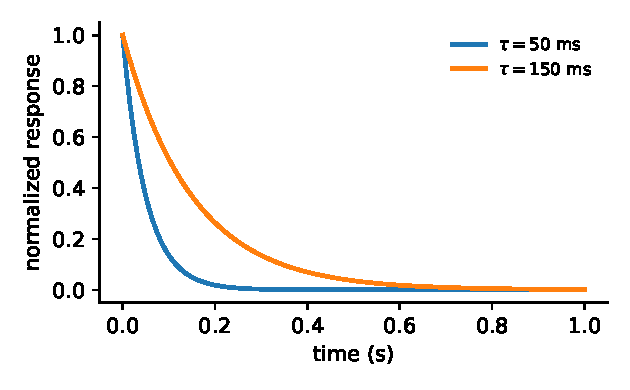
\includegraphics[width=0.5\linewidth]{figures/example-figure}
  \caption{\textbf{Supplementary example figure.} Numbered \cref{fig:supp-example}
    (i.e.\ Fig.~S1), independently of the main-text figures.}
  \label{fig:supp-example}
\end{figure}

\suppsection{Supplementary Tables}
\begin{table}[htbp]
  \centering
  \caption{\textbf{Supplementary example table.} Numbered \cref{tab:supp-example}
    (Table~S1). Parameter tables are the most common supplement in modelling papers.}
  \label{tab:supp-example}
  \begin{tabular}{lcc}
    \toprule
    Parameter & Symbol & Value \\
    \midrule
    Number of neurons   & $N$       & $10\,000$ \\
    Connection density  & $\epsilon$ & $0.1$ \\
    Synaptic delay      & $d$       & $1.5$ ms \\
    \bottomrule
  \end{tabular}
\end{table}

\end{document}
